\documentclass[a4paper,UTF8]{article}
\usepackage{ctex}
\usepackage[margin=1.25in]{geometry}
\usepackage{color}
\usepackage{graphicx}
\usepackage{amssymb}
\usepackage{amsmath}
\usepackage{amsthm}
\usepackage{enumerate}
\usepackage{bm}
\usepackage{hyperref}
\usepackage{epsfig}
\usepackage{color}
\usepackage{mdframed}
\usepackage{lipsum}
\usepackage{mathtools}
\usepackage{hyperref}
\usepackage{diagbox}
\usepackage{float}
\usepackage{caption}
\usepackage{algorithm}
\usepackage{algorithmicx}  
\usepackage{algpseudocode}
\usepackage{amsmath} 
\usepackage{graphicx}
\usepackage{subfigure}
\newmdtheoremenv{thm-box}{myThm}
\newmdtheoremenv{prop-box}{Proposition}
\newmdtheoremenv{def-box}{定义}
\usepackage{listings}
\usepackage{xcolor}
\lstset{
	numbers=left, 
	numberstyle= \tiny, 
	keywordstyle= \color{ blue!70},
	commentstyle= \color{red!50!green!50!blue!50}, 
	frame=shadowbox, % 阴影效果
	rulesepcolor= \color{ red!20!green!20!blue!20} ,
	escapeinside=``, % 英文分号中可写入中文
	xleftmargin=2em,xrightmargin=2em, aboveskip=1em,
	framexleftmargin=2em
} 

\usepackage{booktabs}

\setlength{\evensidemargin}{.25in}
\setlength{\textwidth}{6in}
\setlength{\topmargin}{-0.5in}
\setlength{\topmargin}{-0.5in}

% \setlength{\textheight}{9.5in}
%%%%%%%%%%%%%%%%%%此处用于设置页眉页脚%%%%%%%%%%%%%%%%%%
\usepackage{fancyhdr}                                
\usepackage{lastpage}                                           
\usepackage{layout}                                             
\footskip = 10pt 
\pagestyle{fancy}                    % 设置页眉                 
\lhead{研一下学期}                    
\chead{论文阅读笔记}                                                
% \rhead{第\thepage/\pageref{LastPage}页} 
\rhead{Step4}                                                                                               
\cfoot{\thepage}                                                
\renewcommand{\headrulewidth}{1pt}  			%页眉线宽,设为0可以去页眉线
\setlength{\skip\footins}{0.5cm}    			%脚注与正文的距离           
\renewcommand{\footrulewidth}{0pt}  			%页脚线宽,设为0可以去页脚线

\makeatletter 									%设置双线页眉                                        
\def\headrule{{\if@fancyplain\let\headrulewidth\plainheadrulewidth\fi%
\hrule\@height 1.0pt \@width\headwidth\vskip1pt	%上面线为1pt粗  
\hrule\@height 0.5pt\@width\headwidth  			%下面0.5pt粗            
\vskip-2\headrulewidth\vskip-1pt}      			%两条线的距离1pt        
 \vspace{6mm}}     								%双线与下面正文之间的垂直间距              
\makeatother  

%%%%%%%%%%%%%%%%%%%%%%%%%%%%%%%%%%%%%%%%%%%%%%
\numberwithin{equation}{section}
%\usepackage[thmmarks, amsmath, thref]{ntheorem}
\newtheorem{theorem}{Theorem}
\newtheorem*{definition}{Definition}
\newtheorem*{solution}{Solution}
\newtheorem*{prove}{Proof}
\newcommand{\indep}{\rotatebox[origin=c]{90}{$\models$}}

\usepackage{multirow}

%--

%--
\begin{document}
\title{论文阅读笔记\\
Step4}
\author{MF1833063, 史鹏, spwannasing@gmail.com}
\maketitle

\newpage
\section{Stochastic Answer Networks for Machine Reading Comprehension}
相比以往使用了强化学习的multi-step推理,其独特的特点是在训练过程中,在神经网络的回答模块(最后一层)上使用了一种随机预测dropout。
在训练过程中,我们确定了推理步骤的数目,但在答案模块上执行随机dropout,在解码过程中,我们根据所有步骤的预测平均值来生成答案,而不是最后一步。
\begin{figure}[H]
	\centering
	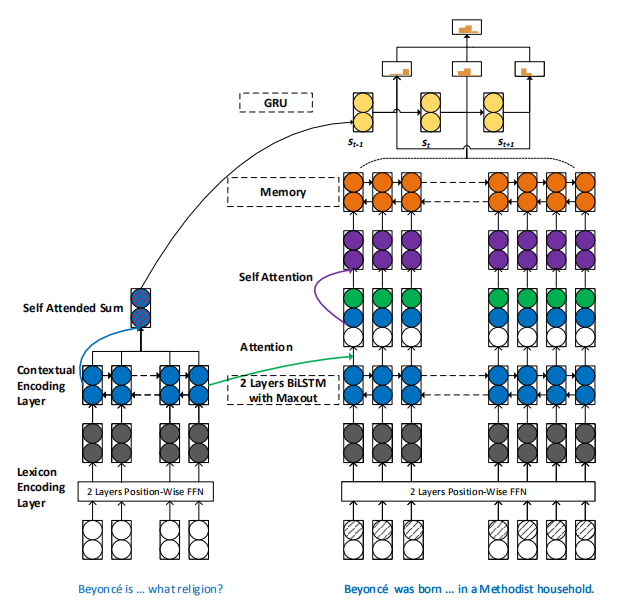
\includegraphics[width=\textwidth]{1-2.png}
\end{figure}
\begin{figure}[H]
	\centering
	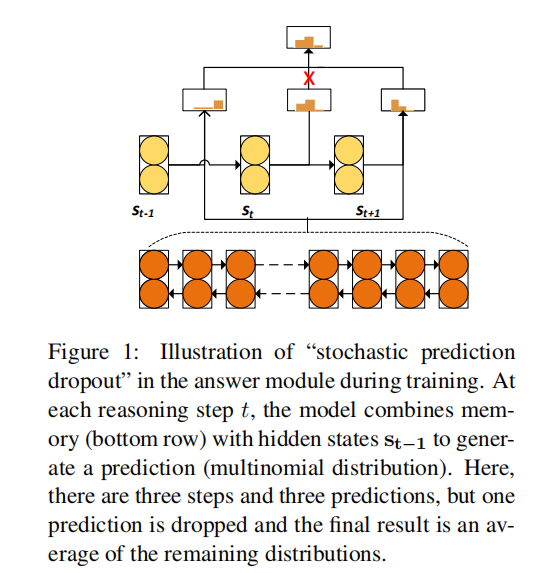
\includegraphics[width=0.6\textwidth]{1-1.png}
\end{figure}
该算法的主要改进就在于answer prediction的过程中。\\
for $t \in\{0,1, \ldots, T-1\}$ \\
\begin{equation}
\begin{array}{c}{P_{t}^{b e g i n}=\operatorname{softmax}\left(s_{t} W_{6} M\right)} \\ {P_{t}^{e n d}=\operatorname{softmax}\left(\left[s_{t} ; \sum_{j} P_{t, j}^{b e g i n} M_{j}\right] W_{7} M\right)}\end{array}
\end{equation}
但是,与其从最后一步输出结果,我们使用所有的输出的平均得分。
\begin{equation}
\begin{array}{c}{P^{b e g i n}=\operatorname{avg}\left(\left[P_{0}^{b e g i n}, P_{1}^{b e g i n}, \ldots, P_{T-1}^{b e g i n}\right]\right)} \\ {P^{e n d}=\operatorname{avg}\left(\left[P_{0}^{e n d}, P_{1}^{e n d}, \ldots, P_{T-1}^{e n d}\right]\right)}\end{array}
\end{equation}
还有个特殊的是,在training的过程中,在averaging操作之前使用随机dropout,能够提升鲁棒性。 
\newpage
\section{Multi-Granularity Hierarchical Attention Fusion Networks for Reading Comprehension and Question Answering}
在所提出的方法中,注意和融合是水平和垂直地跨层进行的,在问题和段落之间的不同粒度级别上进行。
具体来说,它首先用细粒度的语言嵌入对问题和段落进行编码,以便更好地捕捉语义级别上各自的表示。
在此基础上,提出了一种多粒度融合方法,充分融合了全局表示和参与表示的信息。
最后,介绍了一种分层关注网络,该网络以多层次的软度为中心,逐步解决了问题的答案跨度问题。
\begin{figure}[H]
	\centering
	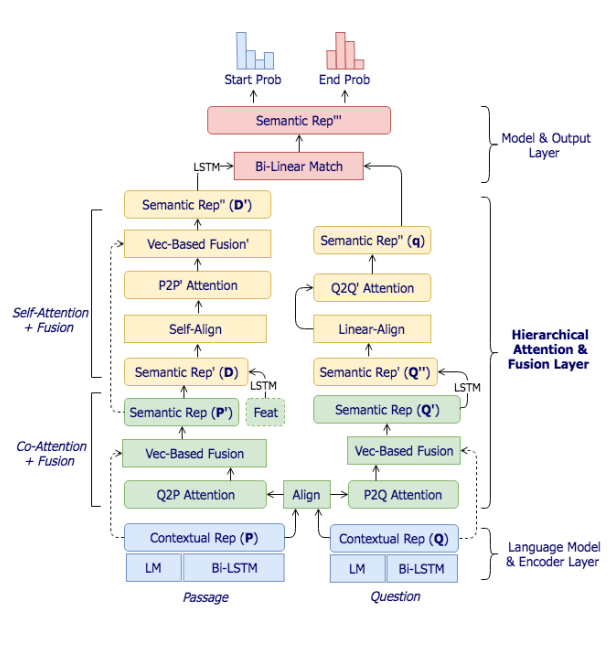
\includegraphics[width=0.8\textwidth]{2-1.png}
\end{figure}

encoder-layer(这里的$c_t$可以看成是residual connection)
\begin{equation}
\begin{aligned} \mathrm{u}_{\mathrm{t}}^{\mathrm{Q}} &=\left[\mathrm{BiLSTMQ}\left(\left[\mathrm{e}_{\mathrm{t}}^{\mathrm{Q}}, \mathrm{c}_{\mathrm{t}}^{\mathrm{Q}}\right]\right), \mathrm{c}_{\mathrm{t}}^{\mathrm{Q}}\right] \\ \mathrm{u}_{\mathrm{t}}^{\mathrm{P}} &=\left[\mathrm{BiLSTM_{P }}\left(\left[\mathrm{e}_{\mathrm{t}}^{\mathrm{P}}, \mathrm{c}_{\mathrm{t}}^{\mathrm{P}}\right]\right), \mathrm{c}_{\mathrm{t}}^{\mathrm{P}}\right] \end{aligned}
\end{equation}

Attention的意义:它的目的是使问题和段落对齐,以便我们能够更好地找到与该问题相关的最相关的passage span。\\

Co-attention\&Fusion:\\
\begin{equation}
	\mathrm{S}_{\mathrm{ij}}=\operatorname{Att}\left(\mathrm{u}_{\mathrm{t}}^{\mathrm{Q}}, \mathrm{u}_{\mathrm{t}}^{\mathrm{P}}\right)=\operatorname{ReLU}\left(\mathrm{W}_{\operatorname{lin}}^{\top} \mathrm{u}_{\mathrm{t}}^{\mathrm{Q}}\right)^{\top} \cdot \operatorname{ReLU}\left(\mathrm{W}_{\operatorname{lin}}^{\top} \mathrm{u}_{\mathrm{t}}^{\mathrm{P}}\right)
	\end{equation}

P2Q Attention:
\begin{equation}
	\alpha_{\mathrm{j}}=\operatorname{softmax}\left(\mathrm{S}_{\mathrm{jj}}\right)
	\end{equation}
	\begin{equation}
		\tilde{\mathrm{Q}}_{ : \mathrm{t}}=\sum_{\mathrm{j}} \alpha_{\mathrm{tj}} \cdot \mathrm{Q}_{ : \mathrm{j}}, \forall \mathrm{j} \in[1, \ldots, \mathrm{m}]
		\end{equation}

Q2P Attention:
\begin{equation}
\begin{array}{c}{\beta_{\mathrm{i}}=\operatorname{softmax}\left(\mathrm{S}_{\mathrm{i} :}\right)} \\ {\tilde{\mathrm{P}}_{\mathrm{k} :}=\sum \beta_{\mathrm{ik}} \cdot \mathrm{P}_{\mathrm{i} :}, \forall \mathrm{i} \in[1, \ldots, \mathrm{n}]}\end{array}
\end{equation}

Fusion:
\begin{equation}
\begin{array}{c}{\mathrm{P}^{\prime}=\text { Fuse }(\mathrm{P}, \tilde{\mathrm{Q}})} \\ {\mathrm{Q}^{\prime}=\text { Fuse }(\mathrm{Q}, \tilde{\mathrm{P}})} \\ {\text { where Fuse }(\cdot, \cdot) \text { is a typical fusion kernel }}\end{array}
\end{equation}

e.g.:
\begin{equation}
	\mathrm{m}(\mathrm{P}, \tilde{\mathrm{Q}})=\tanh \left(\mathrm{W}_{\mathrm{f}}[\mathrm{P} ; \tilde{\mathrm{Q}} ; \mathrm{P} \circ \tilde{\mathrm{Q}} ; \mathrm{P}-\tilde{\mathrm{Q}}]+\mathrm{b}_{\mathrm{f}}\right)
	\end{equation}

Gating Function:
\begin{equation}
\begin{array}{l}{\mathrm{P}^{\prime}=\mathrm{g}(\mathrm{P}, \tilde{\mathrm{Q}}) \cdot \mathrm{m}(\mathrm{P}, \tilde{\mathrm{Q}})+(1-\mathrm{g}(\mathrm{P}, \tilde{\mathrm{Q}})) \cdot \mathrm{P}} \\ {\mathrm{Q}^{\prime}=\mathrm{g}(\mathrm{Q}, \tilde{\mathrm{P}}) \cdot \mathrm{m}(\mathrm{Q}, \tilde{\mathrm{P}})+(1-\mathrm{g}(\mathrm{Q}, \tilde{\mathrm{P}})) \cdot \mathrm{Q}}\end{array}
\end{equation}

Self-attention\&Fusion:
\begin{equation}
	\mathrm{D}=\operatorname{BiLSTM}\left(\left[\mathrm{P}^{\prime} ; \text { feat man }\right]\right)
	\end{equation}
	\begin{equation}
	\begin{array}{c}{\mathrm{L}=\operatorname{softmax}\left(\mathrm{D} \cdot \mathrm{W}_{1} \cdot \mathrm{D}^{\top}\right)} \\ {\tilde{\mathrm{D}}=\mathrm{L} \cdot \mathrm{D}}\end{array}
	\end{equation}
	\begin{equation}
		\mathrm{D}^{\prime}=\mathrm{Fuse}(\mathrm{D}, \tilde{\mathrm{D}})
		\end{equation}
		\begin{equation}
			\mathrm{D}^{\prime \prime}=\operatorname{BiLSTM}\left(\mathrm{D}^{\prime}\right)
			\end{equation}
			\begin{equation}
			\begin{array}{c}{\gamma=\operatorname{softmax}\left(\mathbf{w}_{\mathrm{q}}^{\top} \cdot \mathrm{Q}^{\prime \prime}\right)} \\ {\mathbf{q}=\sum \gamma_{\mathrm{j}} \cdot \mathrm{Q}_{\mathrm{j}}^{\prime \prime}, \forall \mathrm{j} \in[1, \ldots, \mathrm{m}]}\end{array}
			\end{equation}

OutPut:
\begin{equation}
\begin{aligned} \mathrm{P}_{\text { start }} &=\operatorname{softmax}\left(\mathbf{q} \cdot \mathbf{W}_{\mathrm{s}}^{\top} \cdot \mathrm{D}^{\prime \prime}\right) \\ \mathrm{P}_{\text { end }} &=\operatorname{softmax}\left(\mathbf{q} \cdot \mathbf{W}_{\mathrm{e}}^{\top} \cdot \mathrm{D}^{\prime \prime}\right) \end{aligned}
\end{equation}
\begin{equation}
	\mathrm{L}(\theta)=-\frac{1}{\mathrm{N}} \sum_{\mathrm{i}}^{\mathrm{N}} \log \mathrm{p}_{\mathrm{s}}\left(\mathrm{y}_{\mathrm{i}}^{\mathrm{s}}\right)+\log \mathrm{p}_{\mathrm{e}}\left(\mathrm{y}_{\mathrm{i}}^{\mathrm{e}}\right)
	\end{equation}
\newpage
\section{A Multi-Stage Memory Augmented Neural Network for Machine Reading Comprehension}
就是把MemoryNetwork换了一个领域来用。主要去学习Address、read、write的操作。
\begin{figure}[H]
	\centering
	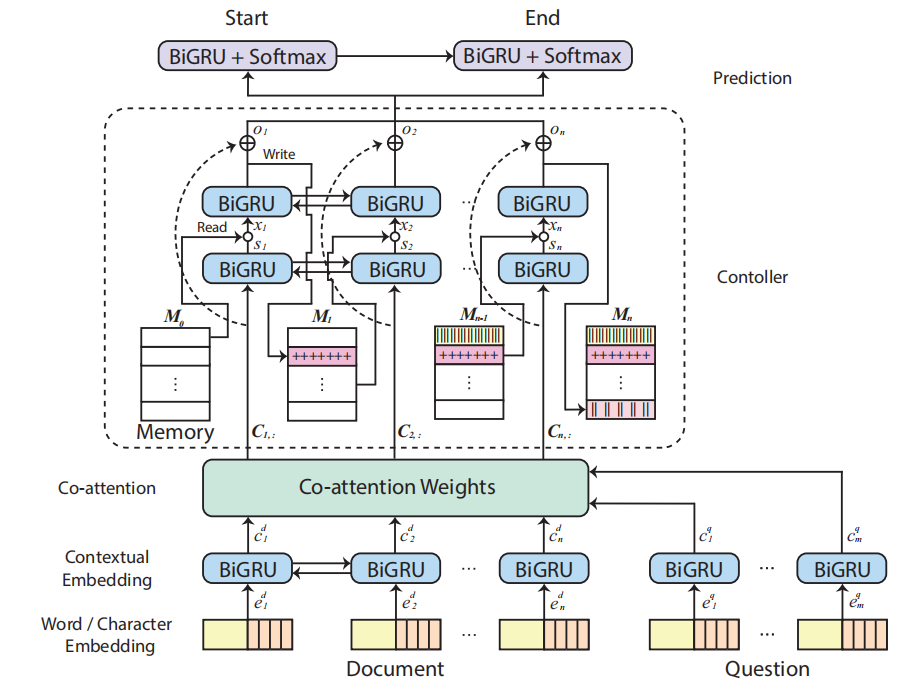
\includegraphics[width=\textwidth]{3-1.png}
\end{figure}
\newpage
\section{S-NET: FROM ANSWER EXTRACTION TO ANSWER GENERATION FOR MACHINE READING COMPREHENSION}
提出了一个extraction-then-synthesis的框架。具体来说,答案提取模型首先用来预测文章中最重要的子区间作为证据,而答案综合模型则以证据作为附加的特征。并附上问题和段落,以进一步详细说明最后的答案。
提出一项额外的passage-ranking任务(Multi-task learning的一次应用),以帮助在多个段落中提取答案。
\begin{figure}[H]
	\centering
	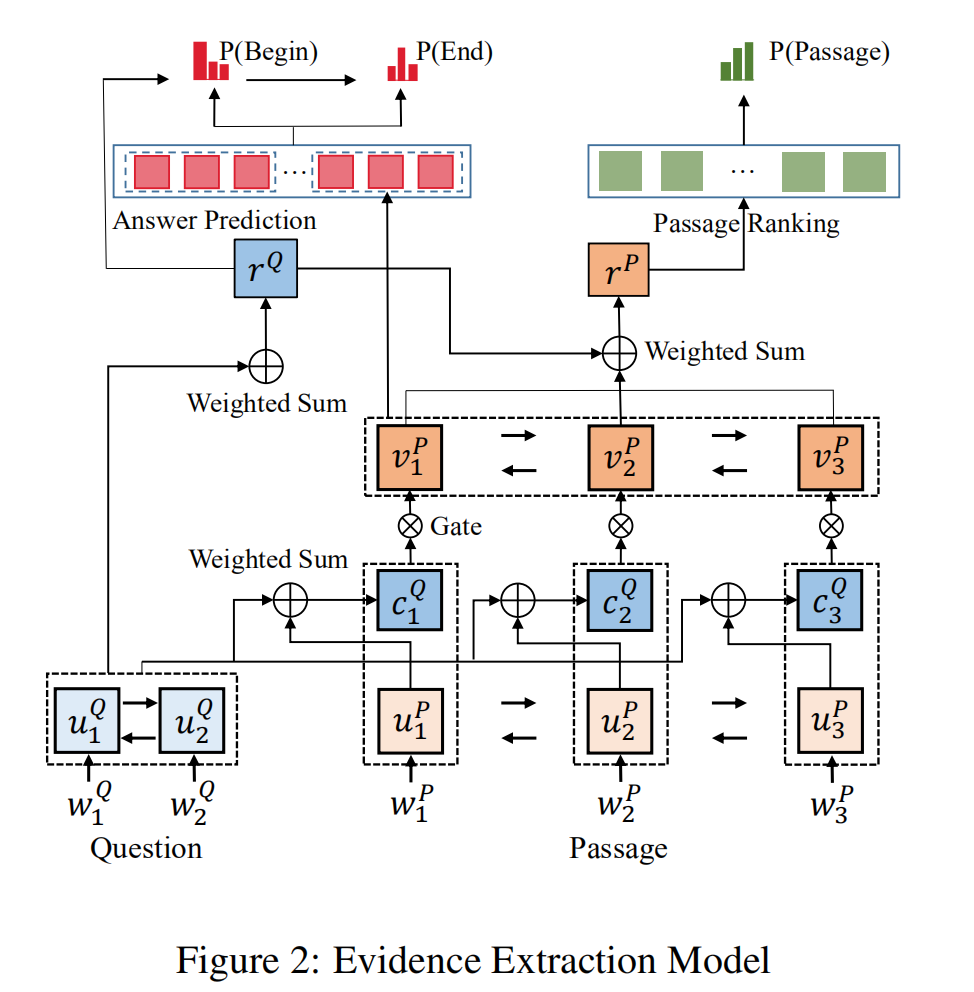
\includegraphics[width=0.65\textwidth]{4-1.png}
\end{figure}
\begin{figure}[H]
	\centering
	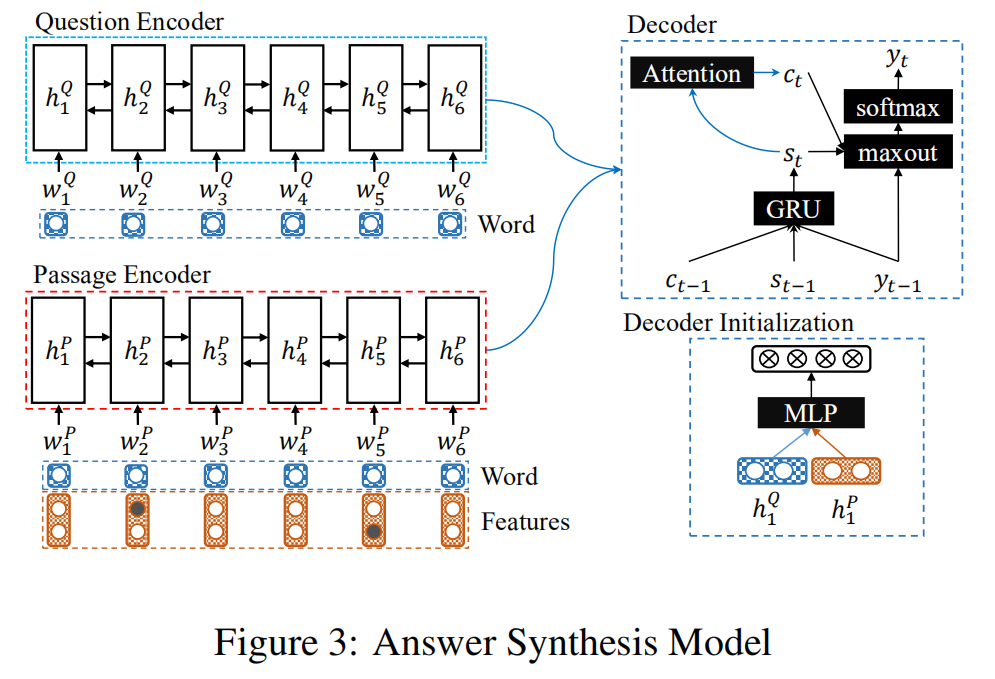
\includegraphics[width=0.65\textwidth]{4-2.png}
\end{figure}
\begin{figure}[H]
	\centering
	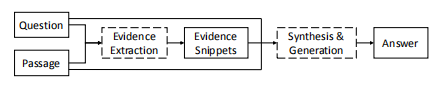
\includegraphics[width=0.6\textwidth]{4-3.png}
	\caption{整体结构}
\end{figure}

EVIDENCE SNIPPET PREDICTION:\\
\begin{equation}
\begin{array}{l}{u_{t}^{Q}=\operatorname{BiGRU}_{Q}\left(u_{t-1}^{Q},\left[e_{t}^{Q}, c h a r_{t}^{Q}\right]\right)} \\ {u_{t}^{P}=\operatorname{BiGRU}_{P}\left(u_{t-1}^{P},\left[e_{t}^{P}, c h a r_{t}^{P}\right]\right)}\end{array}
\end{equation}

attention-pooling vector:
\begin{equation}
\begin{aligned} s_{j}^{t} &=\mathrm{v}^{\mathrm{T}} \tanh \left(W_{u}^{Q} u_{j}^{Q}+W_{u}^{P} u_{t}^{P}\right) \\ a_{i}^{t} &=\exp \left(s_{i}^{t}\right) / \Sigma_{j=1}^{m} \exp \left(s_{j}^{t}\right) \\ c_{t}^{Q} &=\Sigma_{i=1}^{m} a_{i}^{t} u_{i}^{Q} \end{aligned}
\end{equation}

sentence-pair representation:
\begin{equation}
	v_{t}^{P}=\operatorname{GRU}\left(v_{t-1}^{P}, c_{t}^{Q}\right)
	\end{equation}

match-LSTM:
\begin{equation}
\begin{array}{l}{g_{t}=\operatorname{sigmoid}\left(W_{g}\left[u_{t}^{P}, c_{t}^{Q}\right]\right)} \\ {\left[u_{t}^{P}, c_{t}^{Q}\right]^{*}=g_{t} \odot\left[u_{t}^{P}, c_{t}^{Q}\right]} \\ {v_{t}^{P}=\operatorname{GRU}\left(v_{t-1}^{P},\left[u_{t}^{P}, c_{t}^{Q}\right]^{*}\right)}\end{array}
\end{equation}

Answer prediction:
\begin{equation}
\begin{aligned} s_{j}^{t} &=\mathrm{v}^{\mathrm{T}} \tanh \left(W_{h}^{P} v_{j}^{P}+W_{h}^{a} h_{t-1}^{a}\right) \\ a_{i}^{t} &=\exp \left(s_{i}^{t}\right) / \Sigma_{j=1}^{N} \exp \left(s_{j}^{t}\right) \\ p^{t} &=\operatorname{argmax}\left(a_{1}^{t}, \ldots, a_{N}^{t}\right) \end{aligned}
\end{equation}
\begin{equation}
\begin{aligned} c_{t} &=\Sigma_{i=1}^{N} a_{i}^{t} v_{i}^{P} \\ h_{t}^{a} &=\operatorname{GRU}\left(h_{t-1}^{a}, c_{t}\right) \end{aligned}
\end{equation}
\begin{equation}
\begin{aligned} s_{j} &=\mathbf{v}^{\mathrm{T}} \tanh \left(W_{u}^{Q} u_{j}^{Q}+W_{v}^{Q} v_{r}^{Q}\right) \\ a_{i} &=\exp \left(s_{i}\right) / \Sigma_{j=1}^{m} \exp \left(s_{j}\right) \\ r^{Q} &=\sum_{i=1}^{m} a_{i} u_{i}^{Q} \end{aligned}
\end{equation}
\begin{equation}
	\mathcal{L}_{A P}=-\Sigma_{t=1}^{2} \Sigma_{i=1}^{N}\left[y_{i}^{t} \log a_{i}^{t}+\left(1-y_{i}^{t}\right) \log \left(1-a_{i}^{t}\right)\right]
	\end{equation}

Passage ranking:
\begin{equation}
\begin{aligned} s_{j} &=\mathrm{v}^{\mathrm{T}} \tanh \left(W_{v}^{P} v_{j}^{P}+W_{v}^{Q} r^{Q}\right) \\ a_{i} &=\exp \left(s_{i}\right) / \Sigma_{j=1}^{n} \exp \left(s_{j}\right) \\ r^{P} &=\Sigma_{i=1}^{n} a_{i} v_{i}^{P} \end{aligned}
\end{equation}
\begin{equation}
	g=v_{g}^{\mathrm{T}}\left(\tanh \left(W_{g}\left[r^{Q}, r^{P}\right]\right)\right)
	\end{equation}
	\begin{equation}
	\begin{array}{c}{\hat{g}_{i}=\exp \left(g_{i}\right) / \Sigma_{j=1}^{k} \exp \left(g_{j}\right)} \\ {\mathcal{L}_{P R}=-\sum_{i=1}^{k}\left[y_{i} \log \hat{g}_{i}+\left(1-y_{i}\right) \log \left(1-\hat{g}_{i}\right)\right]}\end{array}
	\end{equation}

joint learning:
\begin{equation}
	\mathcal{L}_{E}=r \mathcal{L}_{A P}+(1-r) \mathcal{L}_{P R}
	\end{equation}

ANSWER SYNTHESIS:
\begin{equation}
\begin{array}{l}{h_{t}^{P}=\operatorname{BiGRU}\left(h_{t-1}^{P},\left[e_{t}^{p}, f_{t}^{s}, f_{t}^{e}\right]\right)} \\ {h_{t}^{Q}=\operatorname{BiGRU}\left(h_{t-1}^{Q}, e_{t}^{Q}\right)}\end{array}
\end{equation}
\begin{equation}
\begin{aligned} s_{j}^{t} &=v_{a}^{\mathrm{T}} \tanh \left(W_{a} d_{t-1}+U_{a} h_{j}\right) \\ a_{i}^{t} &=\exp \left(s_{i}^{t}\right) / \Sigma_{j=1}^{n} \exp \left(s_{j}^{t}\right) \\ c_{t} &=\Sigma_{i=1}^{n} a_{i}^{t} h_{i} \end{aligned}
\end{equation}
\begin{equation}
\begin{aligned} d_{t} &=\mathrm{GRU}\left(w_{t-1}, c_{t-1}, d_{t-1}\right) \\ d_{0} &=\tanh \left(W_{d}\left[\overset{\leftarrow}{h}_{1}^{P}, \overset{\leftarrow}{h}_{1}^{Q}\right]+b\right) \end{aligned}
\end{equation}
\begin{equation}
\begin{array}{c}{r_{t}=W_{r} w_{t-1}+U_{r} c_{t}+V_{r} d_{t}} \\ {m_{t}=\left[\max \left\{r_{t, 2 j-1}, r_{t, 2 j}\right\}\right]^{\mathrm{T}}} \\ {p\left(y_{t} | y_{1}, \ldots, y_{t-1}\right)=\operatorname{softmax}\left(W_{o} m_{t}\right)}\end{array}
\end{equation}
\begin{equation}
	\mathcal{L}_{S}=-\frac{1}{|\mathcal{D}|} \Sigma_{(X, Y) \in \mathcal{D}} \log p(Y | X)
	\end{equation}
\newpage
\section{QANET: COMBINING LOCAL CONVOLUTION WITH GLOBAL SELF-ATTENTION FOR READING COMPREHENSION}
本文的创新:\\
1)应该是首先在阅读理解任务上使用了类似Transformer的结构,抛弃了LSTM\\
2)data augmentation,通过back translation来获得更多的训练数据。
\begin{figure}[H]
	\centering
	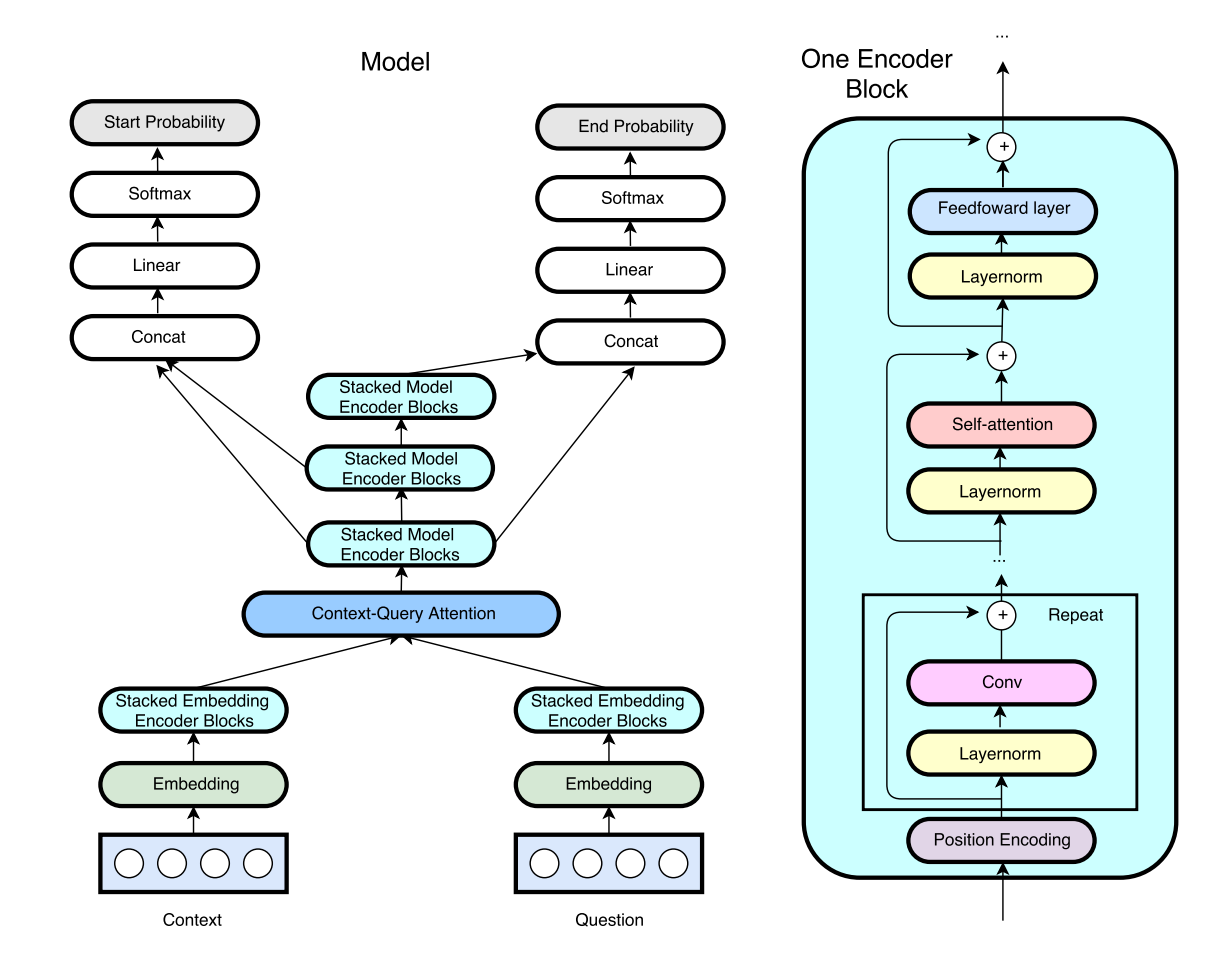
\includegraphics[width=\textwidth]{5-1.png}
\end{figure}
\begin{figure}[H]
	\centering
	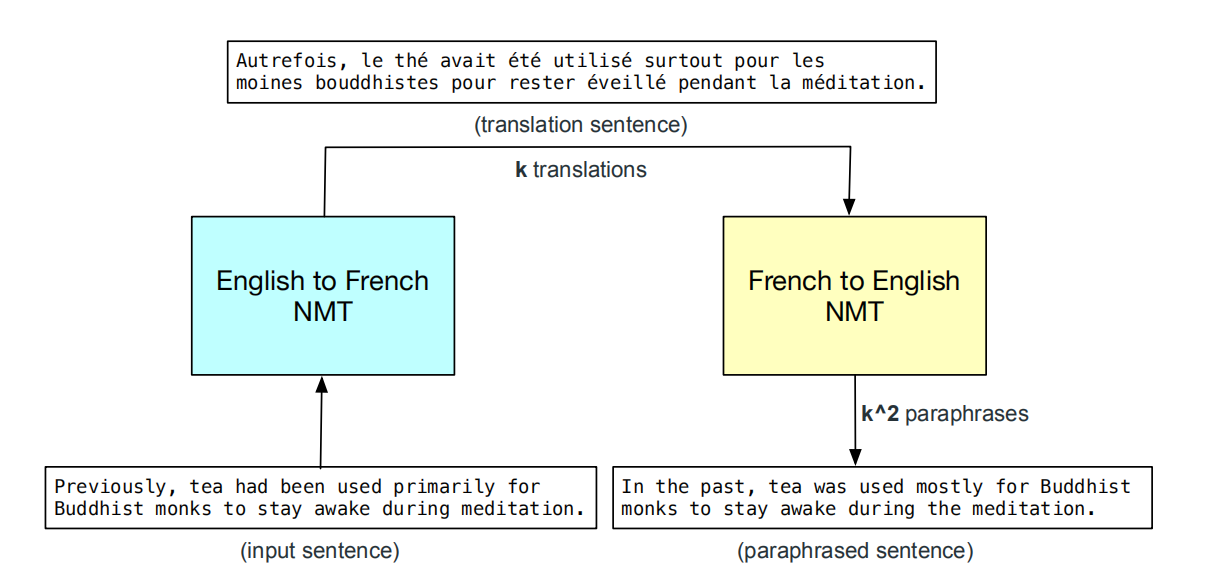
\includegraphics[width=0.7\textwidth]{5-2.png}
\end{figure}
\newpage
\section{Read + Verify: Machine Reading Comprehension with Unanswerable Questions}
机器阅读理解中有无法回答的问题,目的是在无法推断出答案时避免回答。然而,他们无法通过验证预测答案的合法性来验证问题的可回答性。
本文的核心思想是提出了在原始的阅读理解模型的基础上,在预测出答案之后,再verify,重新计算一次No Ansewer的概率。
\begin{figure}[H]
	\centering
	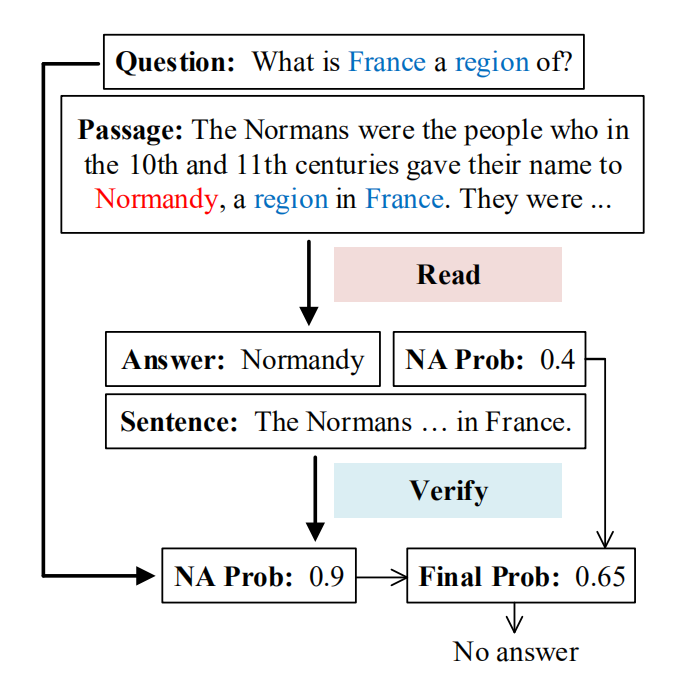
\includegraphics[width=0.6\textwidth]{6-1.png}
\end{figure}
\begin{figure}[H]
	\centering
	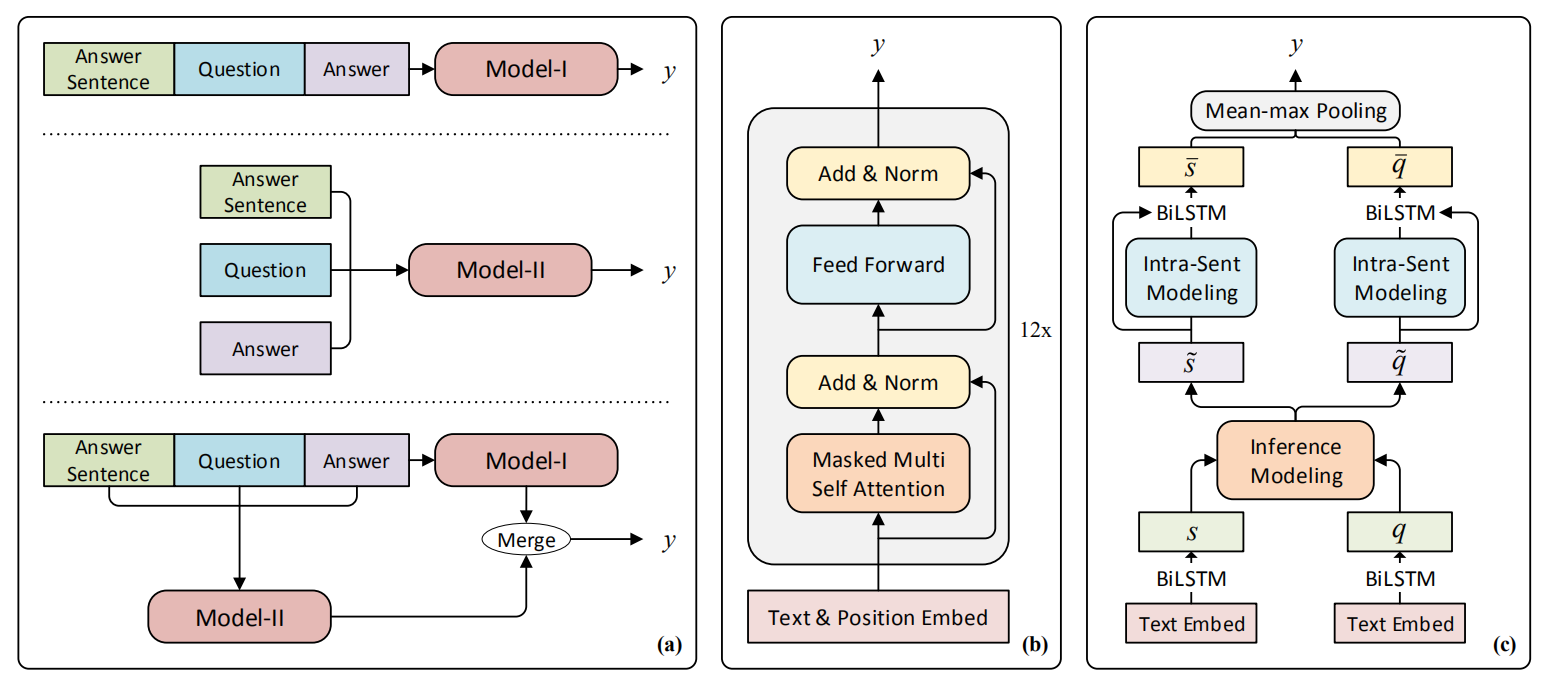
\includegraphics[width=\textwidth]{6-2.png}
\end{figure}
\begin{enumerate}
	\item Reader with Auxiliary Losses
	
\begin{equation}
\begin{array}{c}{o_{j}=w_{v}^{\mathrm{T}} v_{j}, t=\sum_{j=1}^{l_{q}} \frac{e^{o_{j}}}{\sum_{k=1}^{l_{q}} e^{o_{k}}} v_{j}} \\ {\alpha, \beta=\text { pointer network }(U, t)}\end{array}
\end{equation}
\begin{equation}
	\mathcal{L}_{\text {joint}}=-\log \left(\frac{(1-\delta) e^{z}+\delta e^{\alpha_{a} \beta_{b}}}{e^{z}+\sum_{i=1}^{l_{p}} \sum_{j=1}^{l_{p}} e^{\alpha_{i} \beta_{j}}}\right)
	\end{equation}

	\begin{equation}
	\begin{array}{c}{\tilde{o}_{j}=\tilde{w}_{v}^{\mathrm{T}} v_{j}, \tilde{t}=\sum_{j=1}^{l_{q}} \frac{e^{\tilde{\sigma}_{j}}}{\sum_{k=1}^{l_{q}} e^{\tilde{\sigma}_{k}}} v_{j}} \\ {\tilde{\alpha}, \tilde{\beta}=\text { pointer network }(U, \tilde{t})}\end{array}
	\end{equation}
	\begin{equation}
		\mathcal{L}_{\text {indep}-I}=-\log \left(\frac{e^{\tilde{\alpha}_{\overline{a}} \tilde{\beta}_{\overline{b}}}}{\sum_{i=1}^{l_{p}} \sum_{j=1}^{l_{p}} e^{\tilde{\alpha}_{i} \tilde{\beta}_{j}}}\right)
		\end{equation}
		\begin{equation}
			\mathcal{L}_{\text {indep}-I I}=-(1-\delta) \log \sigma(z)-\delta \log (1-\sigma(z))
			\end{equation}
			\begin{equation}
				\mathcal{L}=\mathcal{L}_{j o i n t}+\gamma \mathcal{L}_{i n d e p-I}+\lambda \mathcal{L}_{i n d e p-I I}
				\end{equation}
	\item Answer Verifier
	\subitem[1] Model-I: Sequential Architecture\\
	将answer sentence,question,answer拼起来[S ; Q ; \$ ; A],用GPT的transformer(finetune)来执行此任务。
	\begin{equation}
	\begin{array}{c}{h_{0}=W_{e}[X]+W_{p}} \\ {h_{i}=\text { transformer }_{-} \text { block }\left(h_{i-1}\right), \forall i \in[1, n]}\end{array}
	\end{equation}
	取出最后一层的最后一个token送入linear projection layer
	\begin{equation}
		p(y | X)=\operatorname{softmax}\left(h_{n}^{l_{m}} W_{y}\right)
		\end{equation}
		\begin{equation}
			\mathcal{L}(\theta)=-\sum_{(X, y)} \log p(y | X)
			\end{equation}
	\subitem[2] Model-II: Interactive Architecture
	we use a binary feature to indicate if a word is part of the answer$(fea)$
	\begin{align*}
		s_i &= BiLSTM([word_i^s;char_i^s;fea_i^s]),\forall i \in [1,l_s]\\
		q_i &= BiLSTM([word_j^1;char_j^q;fea_j^q]),\forall j \in [1,l_q]
	\end{align*}
	\begin{equation}
	\begin{array}{c}{a_{i j}=s_{i}^{\top} q_{j}, \forall i \in\left[1, l_{s}\right], \forall j \in\left[1, l_{q}\right]} \\ {b_{i}=\sum_{j=1}^{l_{q}} \frac{e^{a_{i j}}}{\sum_{k=1}^{l_{q}} e^{a_{i k}}} q_{j}, c_{j}=\sum_{i=1}^{l_{s}} \frac{e^{a_{i j}}}{\sum_{k=1}^{l_{s}} e^{a_{k j}}} s_{i}}\end{array}
	\end{equation}
	\begin{equation}
		\tilde{s}_{i}=F\left(s_{i}, b_{i}\right), \tilde{q}_{j}=F\left(q_{j}, c_{j}\right)
		\end{equation}
		\begin{equation}
		\begin{array}{c}{r=\operatorname{gelu}\left(W_{r}[x ; y ; x \circ y ; x-y]\right)} \\ {g=\sigma\left(W_{g}[x ; y ; x \circ y ; x-y]\right)} \\ {o=g \circ r+(1-g) \circ x}\end{array}
		\end{equation}
		\begin{equation}
			\overline{s}_{i}=\operatorname{BiISTM}\left(\left[\tilde{s}_{i} ; \hat{s}_{i}\right]\right), \overline{q}_{j}=\operatorname{BiLSTM}\left(\left[\tilde{q}_{j} ; \hat{q}_{j}\right]\right)
			\end{equation}
	\subitem[3] Model-III: Hybrid Architecture\\
	我们将两个模型的输出向量合并成一个单一的联合表示。然后应用统一的前馈分类器输出无答案概率.这样的设计让我们可以测试从两种不同架构的集成中可以获得更好的性能。在实践中,我们使用一个简单的连接来合并这两个信息源。

\end{enumerate}


\newpage
\section{Adversarial Examples for Evaluating Reading Comprehension Systems}
这篇论文主要就是验证了一个现象,当前的阅读理解模型对于原文添加了一些相关答案的对抗性句子(不违背原意)之后,准确率大幅下降。
\begin{figure}[H]
	\centering
	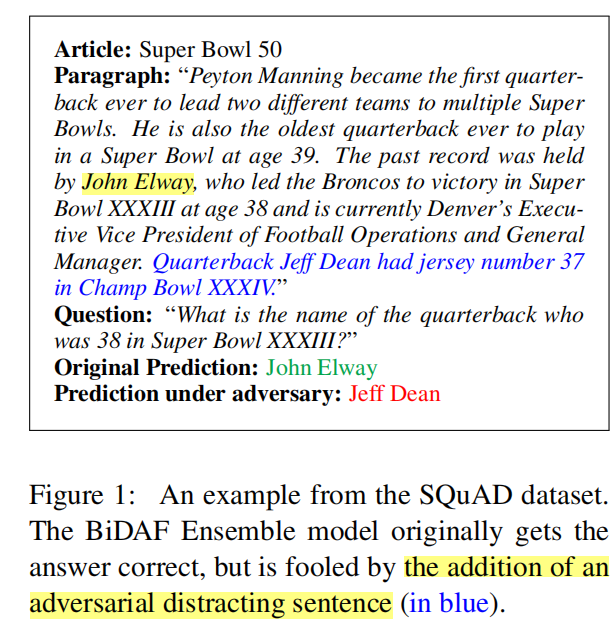
\includegraphics[width=0.6\textwidth]{7-1.png}
\end{figure}
\newpage
\section{Reading Wikipedia to Answer Open-Domain Questions}
主要解决的是开放域问答,在这个论文里即:给出一个问题,从上万个wiki的document中找到答案,核心思想是分为两步,第一步document检索,找到和question最相关的几篇文章,然后第二步在这几篇document上运行常规的MRC算法即可。
我们的方法将基于bigram散列和tf-idf匹配的搜索组件与经过训练以检测维基百科段落中的答案的多层递归神经网络模型相结合。
\begin{figure}[H]
	\centering
	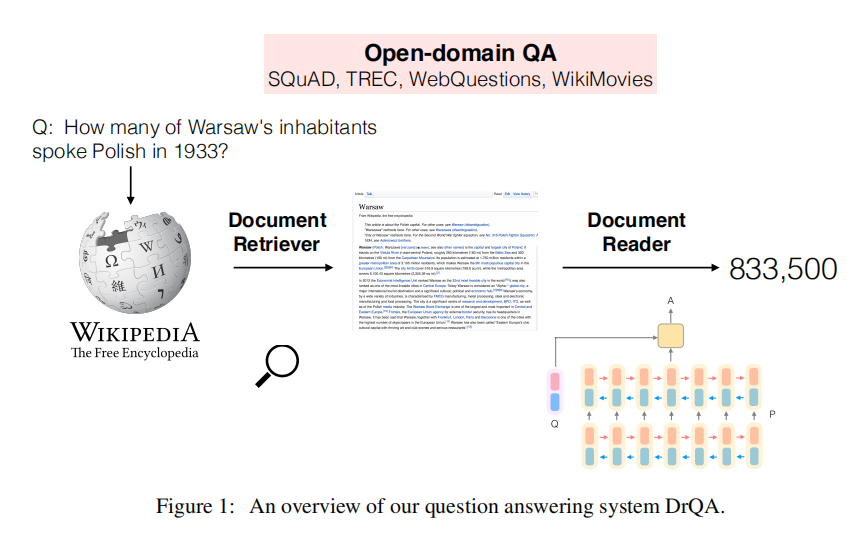
\includegraphics[width=\textwidth]{8-1.png}
\end{figure}
\newpage
\section{DRr-Net: Dynamic Re-read Network for Sentence Semantic Matching}
注意机制在捕捉语义关系和正确对齐两个句子的元素方面起着重要的作用。然而,句子在语义匹配过程中的重要部分随着句子理解程度的变化而动态变化。
因此提出了DRr-Net,每一步都要注意句子的一个小区域,重读重要的单词,以便更好地理解句子的语义。
重点是“Re”的思想,可以借鉴到MRC中。
\begin{figure}[H]
	\centering
	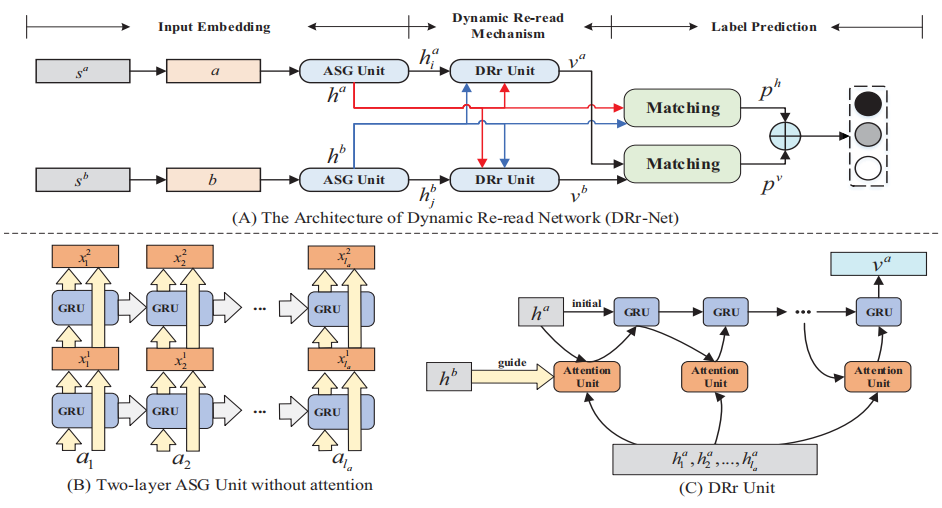
\includegraphics[width=\textwidth]{9-1.png}
\end{figure}

\newpage
\section{FLOWQA: GRASPING FLOW IN HISTORY FORCONVERSATIONAL MACHINE COMPREHENSION}
解决的问题的conversational阅读理解中对于之前的questions的记忆问题,通过“flow”来实现。核心思想是首先1个context对n个问题分别align,
然后经过contextual(bi-lstm)处理后,不同question对应的contex的同一位置的单词送入lstm,即每个lstm处理同一个单词对不同question 的align后的结果。
重复此操作三次。
\begin{figure}[H]
	\centering
	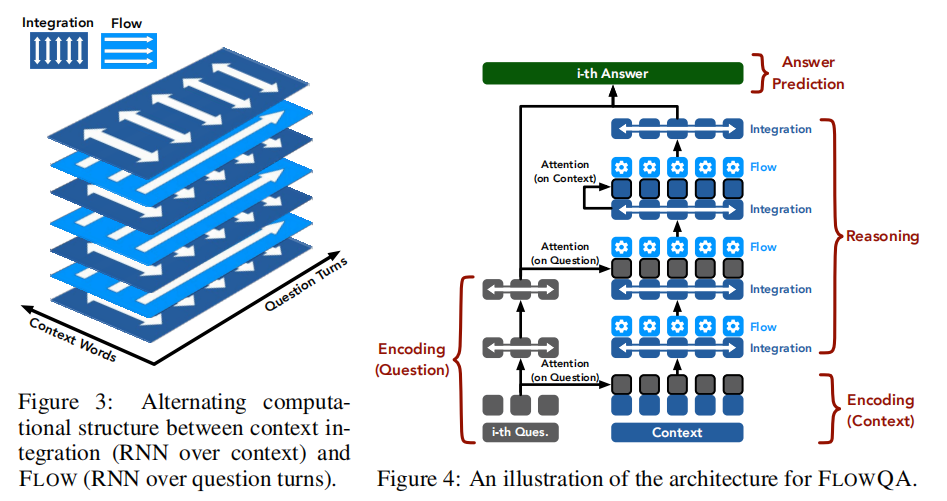
\includegraphics[width=\textwidth]{10-1.png}
\end{figure}
\begin{equation}
	\hat{C}_{i}^{h}=\hat{c}_{i, 1}^{h}, \ldots, \hat{c}_{i, m}^{h}=\operatorname{BiLSTM}\left(\left[\boldsymbol{C}_{i}^{h}\right]\right)
	\end{equation}
	\begin{equation}
		f_{1, j}^{h+1}, \ldots, f_{t, j}^{h+1}=\operatorname{GRU}\left(\hat{c}_{1, j}^{h}, \ldots, \hat{c}_{t, j}^{h}\right)
		\end{equation}
		\begin{equation}
		\begin{array}{c}{F_{i}^{h+1}=\left\{f_{i, 1}^{h+1}, \ldots, f_{i, m}^{h+1}\right\}} \\ {C_{i}^{h+1}=c_{i, 1}^{h+1}, \ldots, c_{i, m}^{h+1}=\left[\hat{c}_{i, 1}^{h} ; f_{i, 1}^{h+1}\right], \ldots,\left[\hat{c}_{i, m}^{h} ; f_{i, m}^{h+1}\right]}\end{array}
		\end{equation}
		\begin{equation}
			Q_{i}^{1}=q_{i, 1}^{1}, \ldots, q_{i, n}^{1}=\operatorname{BiLSTM}\left(Q_{i}\right), Q_{i}^{2}=q_{i, 1}^{2}, \ldots, q_{i, n}^{2}=\operatorname{BiLSTM}\left(Q_{i}^{1}\right)
			\end{equation}
			\begin{equation}
				\tilde{q}_{i}=\sum_{k=1}^{n} \alpha_{i, k} \cdot q_{i, k}^{2}, \alpha_{i, k} \propto \exp \left(w^{T} q_{i, k}^{2}\right)
				\end{equation}
				\begin{equation}
					p_{1}, \ldots, p_{t}=\operatorname{LSTM}\left(\tilde{q}_{i}, \ldots, \tilde{q}_{t}\right)
					\end{equation}
					\begin{equation}
					\begin{aligned} C_{i}^{1} &=\operatorname{IF}\left(C_{i}^{0}\right) \\ C_{i}^{2} &=\operatorname{IF}\left(C_{i}^{1}\right) \end{aligned}
					\end{equation}
					\begin{equation}
						\hat{q}_{i, j}=\sum_{k=1}^{n} \alpha^{i, j, k} \cdot q_{i, k}^{2}, \alpha^{i, j, k} \propto \exp \left(S\left(\left[c_{i} ; c_{j, i}^{1} ; c_{j, i}^{2}\right],\left[q_{j, k} ; q_{j, k}^{1} ; q_{j, k}^{2}\right]\right)\right)
						\end{equation}
						\begin{equation}
							C_{i}^{3}=\operatorname{IF}\left(\left[c_{i, 1}^{2} ; \hat{q}_{i, 1}\right], \ldots,\left[c_{i, m}^{2} ; \hat{q}_{i, m}\right]\right)
							\end{equation}
							\begin{equation}
								\hat{c}_{i, j}=\sum_{k=1}^{m} \alpha^{i, j, k} \cdot c_{i, k}^{3}, \alpha^{i, j, k} \propto \exp \left(S\left(\left[c_{i, j}^{1} ; c_{i, j}^{2}, c_{i, j}^{3}\right],\left[c_{i, k}^{1} ; c_{i, k}^{2}, c_{i, k}^{3}\right]\right)\right)
								\end{equation}
								\begin{equation}
									C_{i}^{4}=\operatorname{BiLSTM}\left(\left[c_{i, 1}^{3} ; \hat{c}_{i, 1}\right], \ldots,\left[c_{i, m}^{3} ; \hat{c}_{i, m}\right]\right)
									\end{equation}
\end{document}